\chapter{Results}
 
\section{Pion Spectra}
\label{sec:pionSpectra}

To correct for the efficiency, we apply a track-by-track correction, where the efficiency of the i-th track $\epsilon_i$ is retrieved from the database, from the parameters discussed in Section~\ref{sec:efficiency}. The correction factor $C_i$ is then defined as,

\begin{equation}
C_i = \epsilon_i^{-1}.
\end{equation}

Each track that is identified as a pion as describe in Section~\ref{sec:pid}, is then weighted by the correction factor $C_i$, when filling the histogram of any observable. In this way, we can correct for the efficiency of the track into any observable of interest, notably transforming from the lab frame into the center-of-mass (CM) frame. Before performing the transformation to the CM system, recall there is a small, but non-negligible, beam angle in the Lab frame; see Section~\ref{sec:beamangle}. The beam angle for each event is measured by the beam tracking software and a rotation is applied to all the tracks in an event, to align the beam angle along the z-axis. Doing so makes the transformation into the CM system much simpler to describe. If the beam direction is defined by a unit vector $\hat{b}$, we can define the rotation that rotates the beam into the z-axis as a rotation about an arbitrary vector $\hat{v} = \hat{b}\times\hat{z}$ where the angle between the two is given by $\cos \theta = \hat{b}\cdot\hat{z}$. A rotation is then applied around the vector $\hat{v}$.

Once all the events have been rotated to align with the z-axis, transforming from the Lab to the CM frame is done by a Lorentz transformation. The 4-momentum vector in the lab frame is defined as $\textbf{P} = (E/c,p_x,p_y,p_z)$. Where the corresponding Lorentz transform into the CM frame along the beam (z-axis) is defined as,

\begin{equation}
A = \begin{pmatrix}
1 & 0 & 0 & 0\\
0 & 1 & 0 & 0\\
0 & 0 & \gamma & -\beta \gamma\\
0 & 0 & -\beta \gamma & \gamma
\end{pmatrix},
\end{equation}

where $\beta$, describes the velocity of the CM system, and $\gamma=\sqrt{1-\beta^2}^{-1}$. The parameter $\beta$ can be determined from the total momentum of the system in the Laboratory frame $P = \sqrt{ T_{P}^2 - M_{T}^2}$ and the total energy of the system $E = T_{P} + M_{P} + M_{T}$ as $\beta = -P/E$, where the (-) sign denotes the correct direction for transforming from the Lab to the CM frame. The CM transformed track is defined as $p^{CM} = \textbf{A}p^{Lab}$.

\begin{figure}[!htb]
\centering
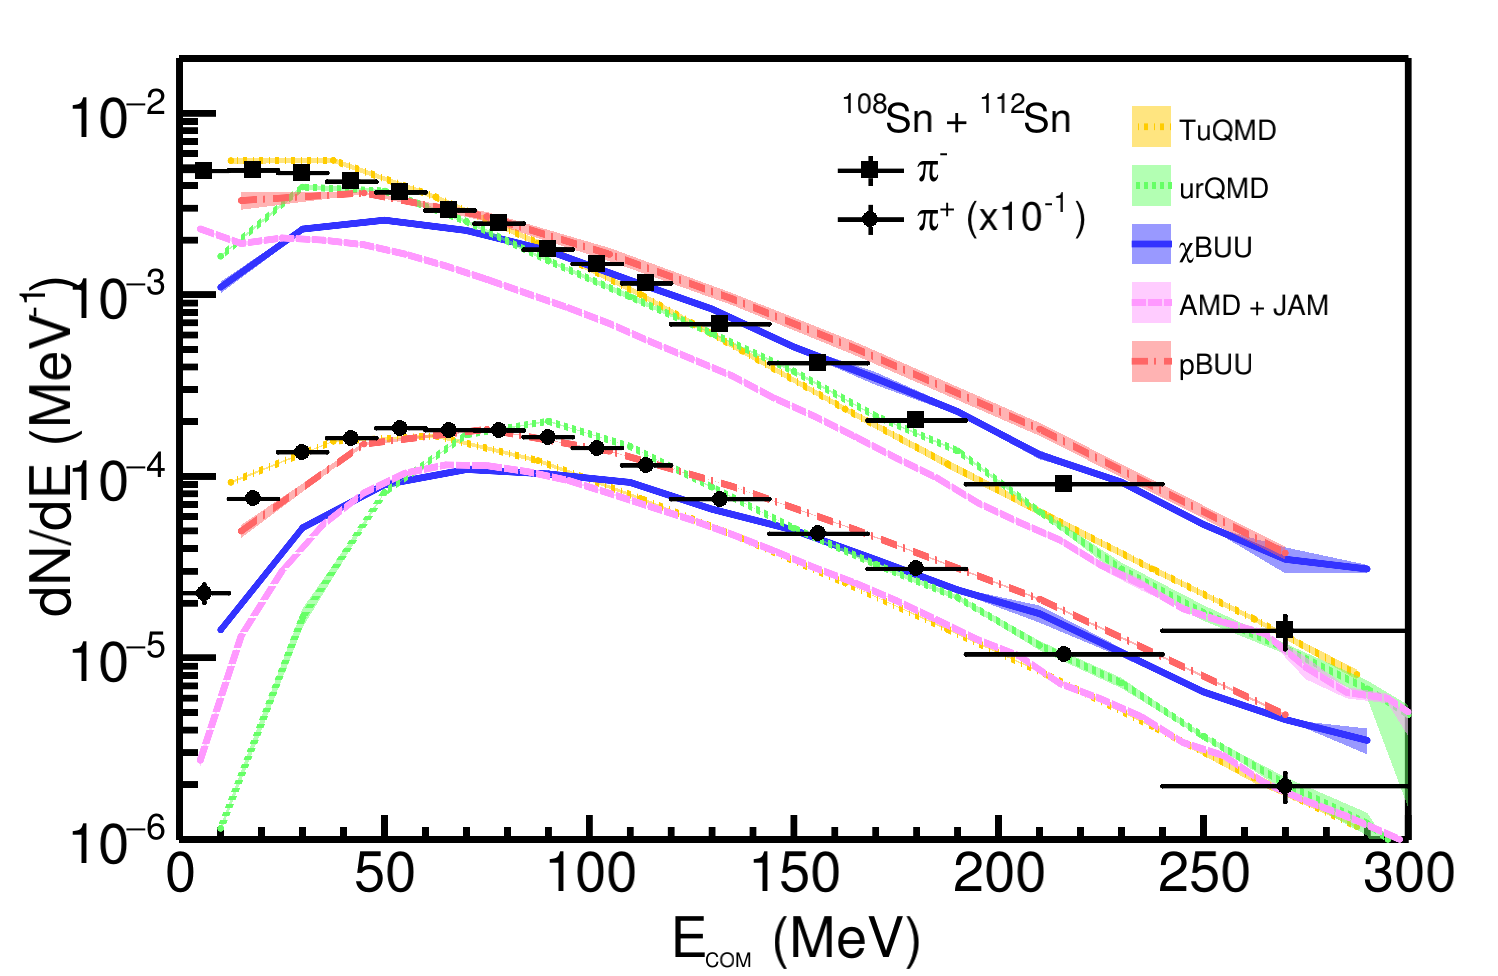
\includegraphics[width=\textwidth]{pionSpectra.png}
\caption{Pion spectra. }
\label{fig:pionspectra}
\end{figure}
%need to add error analysis
%systematic error analysis


Figure~\ref{fig:pionspectra} shows pion CM kinetic energy spectra for both the $\tin{132}{124}$ and $\tin{108}{112}$ systems; corrected for efficiency and accounting for the solid angle of 4$\pi$. This data marks the first time pion spectral data  has been measured at sub-threshold energies. In the pion spectra, we can see the effect of the coulomb potential, which accelerates $\pi^+$ and decelerate $\pi^-$ particles, due to the positive charge of the nuclear medium. The low $\pi^+$ production at low energy is caused by the coulomb barrier between protons. The effects of the Coulomb force are the largest effects on the spectra of the pions and will play an important role when looking at pion spectral ratios. 



%Add figure on Glauber model 
%Add figure on comparison to FOPI data



\section{Comparison to Theory}
%Add figure of Pion spectra for different theory 
%Reference paper for multiple theories

The data taken has been compared with 7 commonly used transport theoretical codes. These codes took part in a large collaborative effort in order to standarize certain common elements of each codes. Each comparison project simulating nuclear matter in a box type simulation with fixed, well defined, initial conditions. Though not physical, this provided a benchmark for codes to compare to; the solutions of the total number of pions and $\Delta$ produced had an analytical solution one would expect from statistical equalibrium, providing a good benchmark. This allowed for each code to systematically go through the numerical treatment and details in each code such as intialization of nuclei, stability of the code, numerical handing of pauli-blocking, etc. \cite{theoryComp1,theoryComp2}. These codes were taken in their best configuration, as a result of these comparison projects, without any prior knowledge of the experimental data. We then simulated the 4 systems measured in the \spirit TPC at an impact parameter of \SI{3}{\femto\metre} at \SI{270}{\MeVA} beam energy. While numerical treatments of each code are resonably similar, each code differs in its treatment of pion and $\Delta$ dynamics. Some codes contain modifications to how the pion behaves in nuclear matter, i.e. \emph{in-medium effects}, typically introduced by including a pion optical potential which describes the pion scattering and absorptions. Some codes include the iso-scalar and the iso-vector delta potential, which are not very well constrained but are important in the production of pions CITE HERE. The set of 7 codes represent the best codes which can simulate pions at these energies. As will be the re-occuring theme, there is a large variation between theoretical codes; greater than the variation between different symmetry energy in a particular code. Though many of the numerical and theoretical treatments have been addressed, many of the details of pion production and dynamics have not been addressed. This is an extremely complex task requiring major theoretical efforts and new data. We expect the data in this thesis and in \cite{jon} to provide much needed experimental data in which each code may compare too. The total theoretical uncertainty is too large relative to the experimental error bars to make a constraint on the density dependence of the symmetry energy. Any constraint would depend on the particular code one is using and would result in conflicting conclusions when using another theory. There is no good consensus at this time which codes should be favored over other codes, as the magnitude of the effects included in each code are still debated in order of importance. Here I will present the current level of agreement with the codes and remark on some of the implications it has moving forward. 


\section{Pion Yield}

The integrated pion yield for both systems, and the $\pi^-/\pi^+$ ratio, is listed in Table~\ref{tb:pionyield}, where the systematic errors are the first error bar and the statistical error is listed next. It is remarkable that the pion ratio is significantly greater than the $N/Z$ of the system, as expected in the Delta Resonance model or under the assumption of chemical equilibrium which is $\pi^-/\pi^+ = (N/Z)^2$ \cite{baoan_piprod1,baoan_piprod2}. In the $\tin{132}{124}$ system this is a factor of 2 times greater and in $\tin{108}{112}$ the system a factor of 1.4 times greater. The pion ratio was hypothesized to be proportional to the high density N/Z ratio of the early system, where the other effects such as pion absorption and re-emission would dilute the effect, lowering the pion ratio as the system tends toward isospin equilibrium. A na\"ive interpretation would be the high density N/Z fraction is much higher than the average of the target and projectile, though, the system spends very little time in this early high density phase and there is really no time for the system to evole such that it could be enhanced in neutron fraction. A more likely conclusion is the mechanisms involved in pion productions via the $\Delta(1232)$ resonance is more complicated than the simple $(N/Z)^2$ relation, which was also seen in \cite{fopi}. Some codes assume the potential of the delta is just the same as the corresponding nucleon potential, as given by the iso-spin. Other codes introduce $\Delta$ resonance in-medium potential, which has an iso-scalar component (independent of iso-spin) and an iso-vector component.  The nature of these two potentials is still unknown, and the role it plays in pion production has shown to be very important \cite{baoan_deltapotential}.


\begin{table*}\centering
\ra{1.3}
\begin{tabular}{@{}cccc@{}}\toprule
System & $\pi^-$ & $\pi^+$ & $Y(\pi^-)/Y(\pi^+)$  \\
\midrule
$\tin{132}{124}$ & 0.717(24)(4) & 0.148(5)(2) & 4.84(10)(6)  \\
$\tin{108}{112}$ & 0.399(14)(3) & 0.200(8)(2) & 1.99(4)(3)  \\
%$\tin{132}{124}$ & \numerr{0.717}{0.024}{0.004} & \numerr{0.148}{0.005}{0.002} & \numerr{4.84}{0.10}{0.06}  \\
%$\tin{108}{112}$ & \numerr{0.399}{0.014}{0.003} & \numerr{0.200}{0.008}{0.002} & \numerr{1.99}{0.04}{0.03}  \\
\bottomrule
\end{tabular}
\caption{Total pion yield.}
\label{tb:pionyield}
\end{table*}


We have compared the total pion yields and ratios to the 7 common transport codes for the systems measured. The table of the transport codes are listed in Appendix~\ref{tb:pionyieldTheory}. Figure~\ref{fig:totalpiYield} shows the total pion yield for the four systems measured as compared with the codes. The codes plotted here are only the soft symmetry energy since the variation in code is much larger than the variation within a code between different symmetry energies. While some codes make a reasonable approximation of a particular charge pion yields, no code reasonably predicts both. 

\begin{figure}[!htb]
\centering
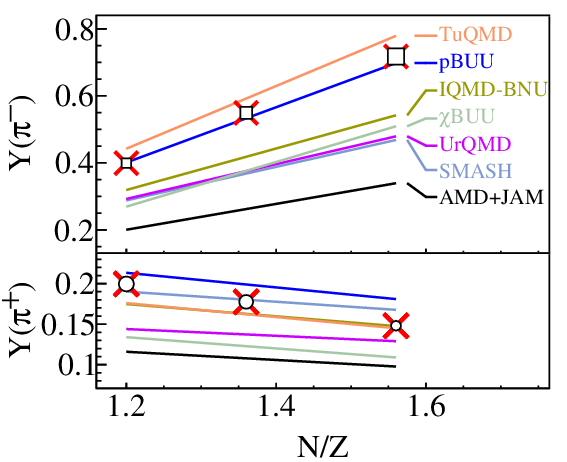
\includegraphics[width=.8\textwidth]{totalpiYield.png}
\caption{Total pion yields as compared with 6 common transport codes.}
\label{fig:totalpiYield}
\end{figure}

Figure~\ref{fig:totalpiRatio} shows the total single pion ratio and the double ratio of the $\tin{132}{124}$ and $\tin{108}{112}$ system. Here, the variation between codes is much larger than the variation between the symmetry energy within a particular code. The symmetry energy variation (soft and stiff extremes) of two codes -- $\chi$BUU and TuQMD -- is plotted as a wide band in the single ratio and in all codes in the double ratio. The data ciruclar markers and band represents the total error bar. Certainly the variation between symmetry energy extremes in the codes, though small, still exists; as initially predicted \cite{baoan_piprod1,baoan_piprod2}. The small error bars in the data would facilitate a detailed analysis to extract the high density behavior of the symmetry energy, if not for large variation between codes. 



\begin{figure}[!htb]
\centering
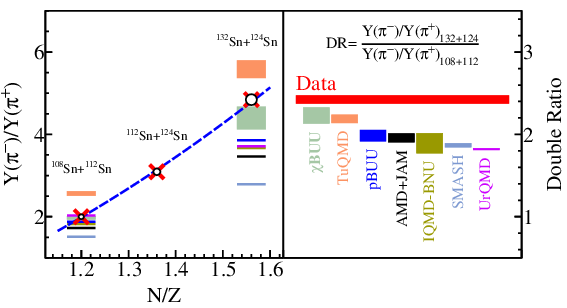
\includegraphics[width=\textwidth]{totalpiRatio.png}
\caption{Total pion ratio and double ratio compared with 7 common transport codes.}
\label{fig:totalpiRatio}
\end{figure}



\section{Pion Spectral Ratio}


\begin{figure}[!htb]
\centering
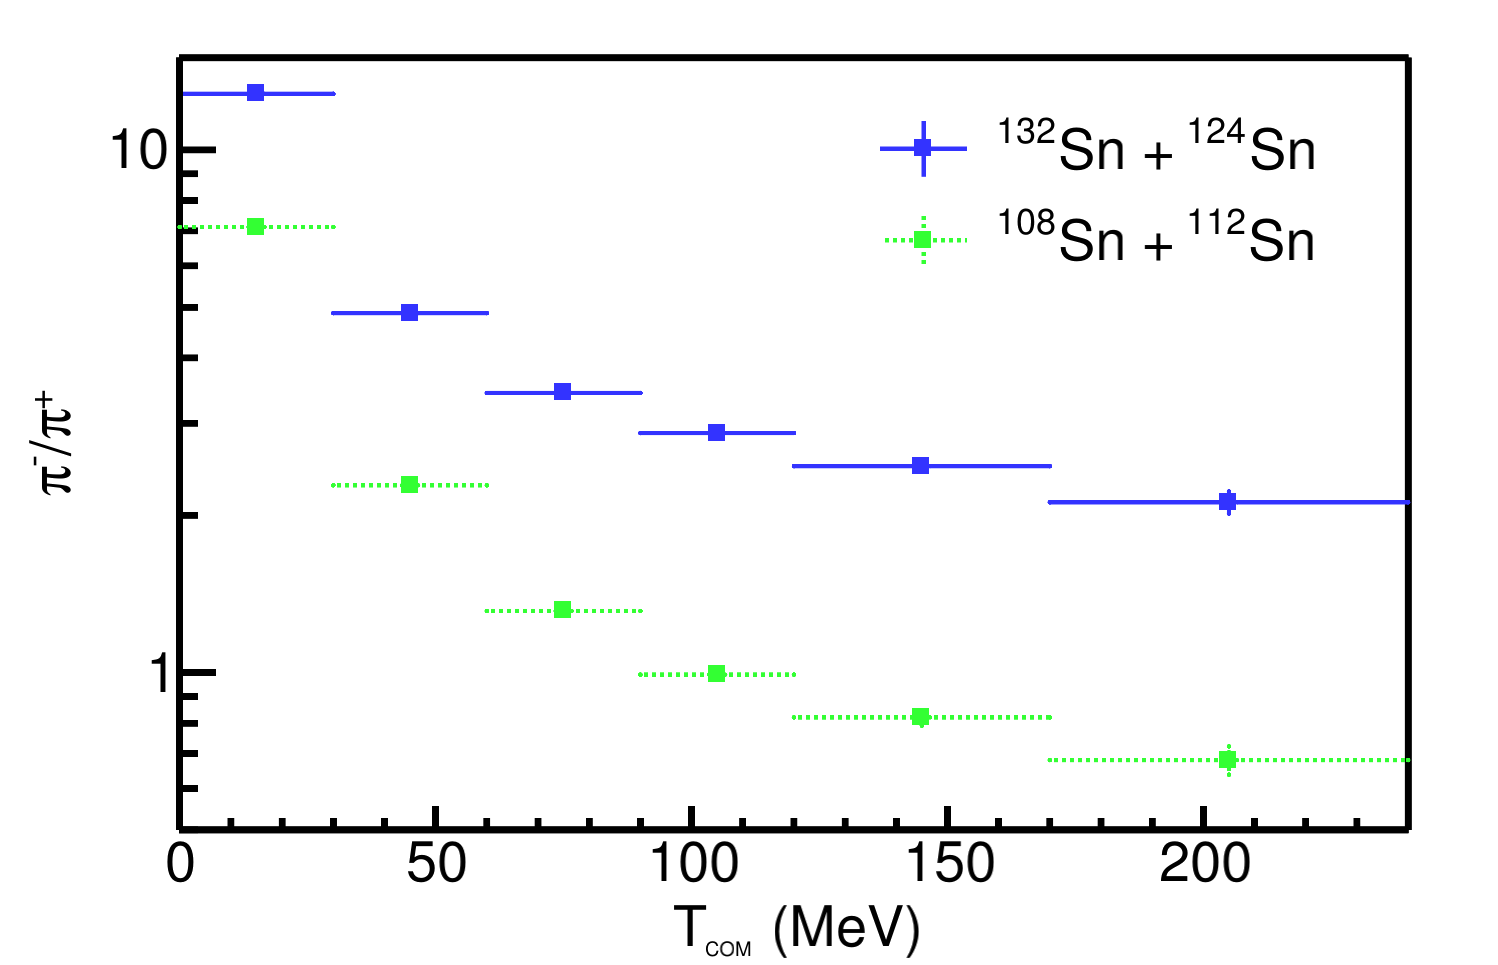
\includegraphics[width=\textwidth]{singleRatio.png}
\caption{Single ratio spectra}
\label{fig:SRspectra}
\end{figure}

The pion spectral ratio is a rather promising observable. In particular it may be more sensitive to the high density regions of the early collision. In theory the high energy pions are more likely to exit the nuclear medium earlier, and therefore be less prone to effects such as pion absorption and re-emission which dilute the sensitivity of the pion observable to the high density behavior. Also low energy pions are more likely to be affected by other effects such as the $\Delta$ potential in medium \cite{baoan_deltapotential}. If we integrate the total pion yield we would combine these two regions diluting the observable. Instead we can construct the $Y(\pi^-)/Y(\pi^+)$ ratio as a function of the kinetic energy in the CM system with a particular focus on high energy pions.

%Mention and cite appendix for systematics

Figure~\ref{fig:SRspectra} shows the pion spectral ratio for both systems, which was measured with a high degree of efficiency and accuracy. The general hyperbolic shape arises from the Coulomb force on the two charged pion spectra mentioned in Section~\ref{sec:pionSpectra}. Also notice the pion ratio is smaller for less neutron poor system, as we would expect since less neutron-neutron collisions produce less $\pi^-$. The bin size of the last bin was increased to reduce the statistical error bars since the number of pions, especially the $\pi^+$, reaches the limits of the measured distribution. 



%Add figure of Theory for pion ratios

\section{Pion Double Ratio}
%Add figure of Theory for pion ratios

\begin{figure}[!htb]
\centering
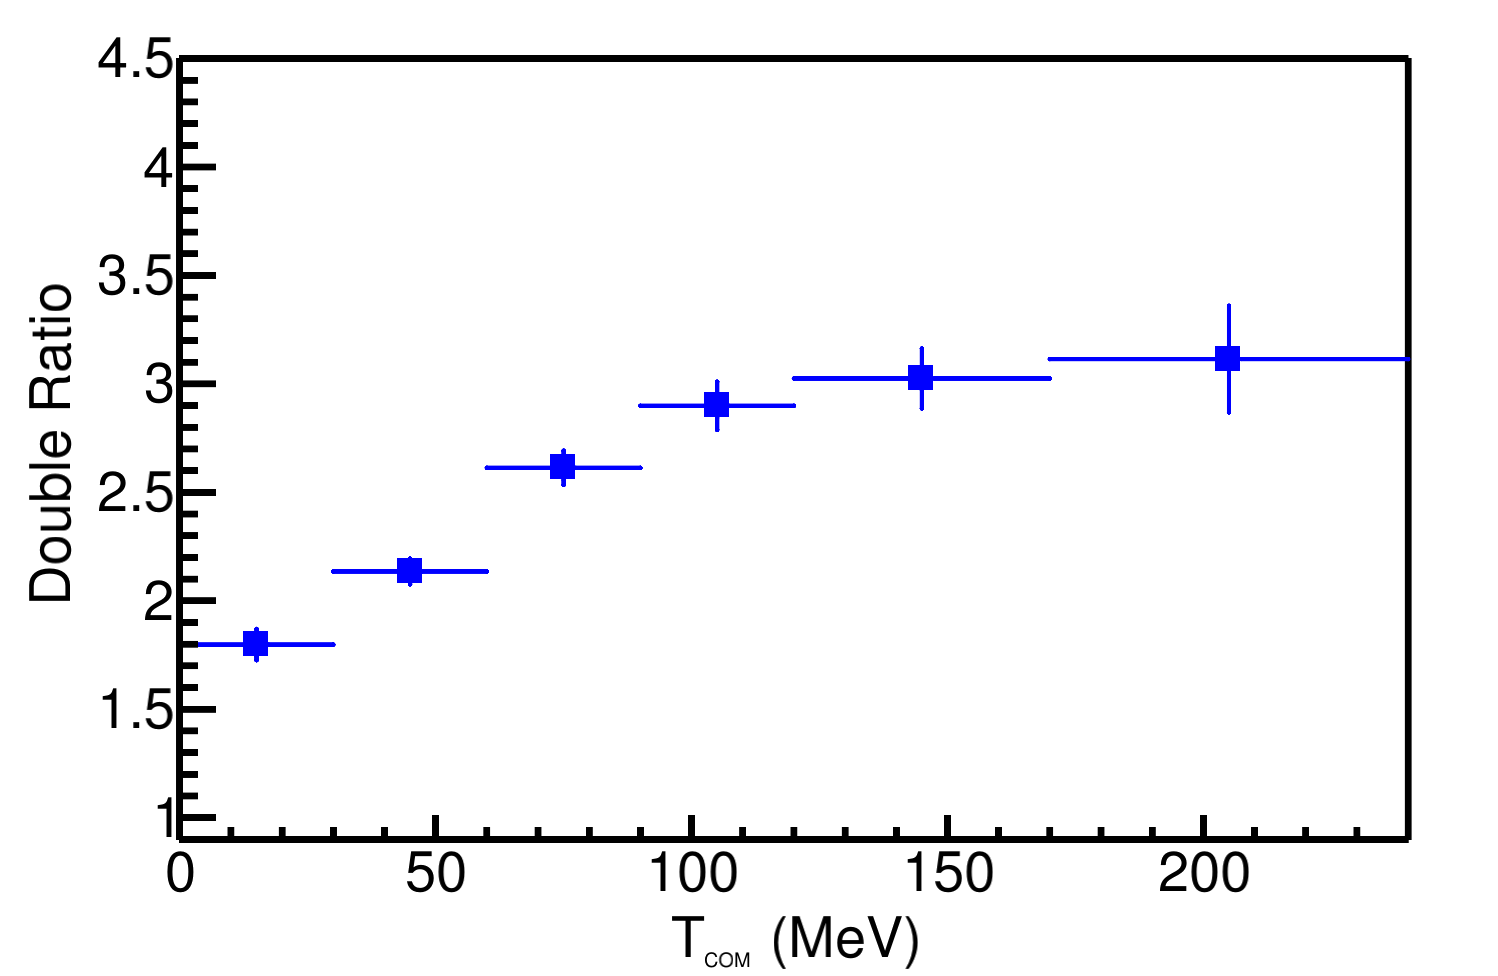
\includegraphics[width=\textwidth]{doubleRatio.png}
\caption{}
\label{fig:spectraDR}
\end{figure}

Another promising observable is the spectral double ratio. In a similar way described in Section~\ref{sec:doubleRatio} we would expect systematic uncertainties in the experiment, and even in the theory, to cancel out. For the same reasons as the pion spectral ratio, we would expect the high energy pions to be more sensitive to the high density region of the early collision. 



\section{Comparison to Previous Data Sets (FOPI)}


\begin{figure}[!htb]
\centering
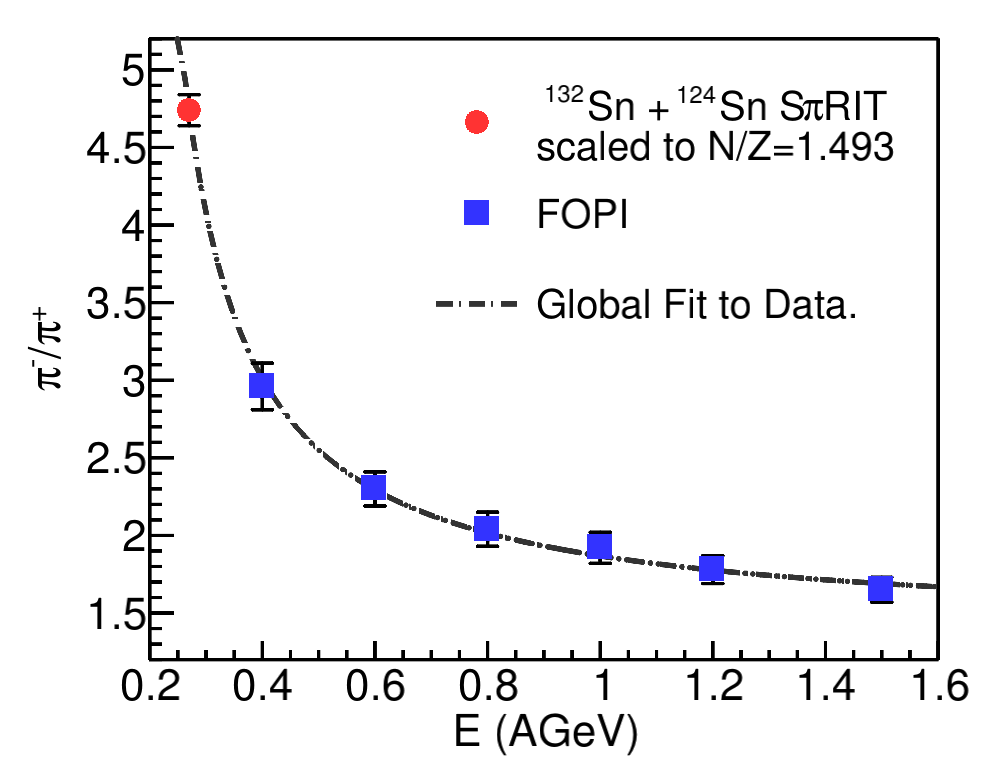
\includegraphics[scale=.4]{fopi_pionratio_comp}
\caption{Comparing the total $\pi^-/\pi^+$ ratio of the $\tin{132}{124}$ system to the ${}^{197}$Au + ${}^{197}$Au data from the FOPI collaboration. The \spirit TPC data was scaled by a factor to compare to the lower N/Z of the Au + Au system. This was extracted from measuring the N/Z dependence measured in the experiment. }
\label{fig:fopiPionRatio}
\end{figure}

The FOPI collaboration has measured the total pion multiplicity resulting from ${}^{197}Au + {}^{197}Au$ collisions at several, higher, beam energies. In the $\tin{132}{124}$ data the $N/Z=1.56$ where as in the ${}^{197}Au + {}^{197}Au$ the $N/Z=1.493$. We also expect the pion ratio is proportional to the $N/Z$ of the system. Since 4 beams were measured in this experiment, the $N/Z$ dependence was measured as seen in Fig.~\ref{fig:totalpiRatio}. Here the dependence is fitted with a 2-nd order polynomial fit. To compare the pion ratio in the $\tin{132}{124}$ data with that of the lower N/Z in the FOPI experiment, we scaled by the pion ratio between $N/Z=1.56$ and 1.493 as given from the fitted polynomial line. Figure~\ref{fig:fopiPionRatio} shows the scaled pion ratio as compared with the FOPI pion ratio \cite{fopi}. The fitted function has the functional form of $p_1(E - p_2)^{-2}$ where $p_1$ and $p_2$ are free parameters, and only is meant to guide the eye. It is also worth mentioning that the pion ratio observed in the FOPI \SI{400}{\MeVA} setting was already considerably higher than what is expected from the $(N/Z)^2$ delta resonance model \cite{baoan_piprod1,baoan_piprod2}. Scaling the other systems in the \spirit TPC data leads to almost the exact same value of $\mathrm{Y}(\pi^-)/\mathrm{Y}(\pi^+) = \num{4.82}$ and would be redundant. 






